\documentclass[class=article, crop=false]{standalone}
\usepackage{my_preamble}
\begin{document}
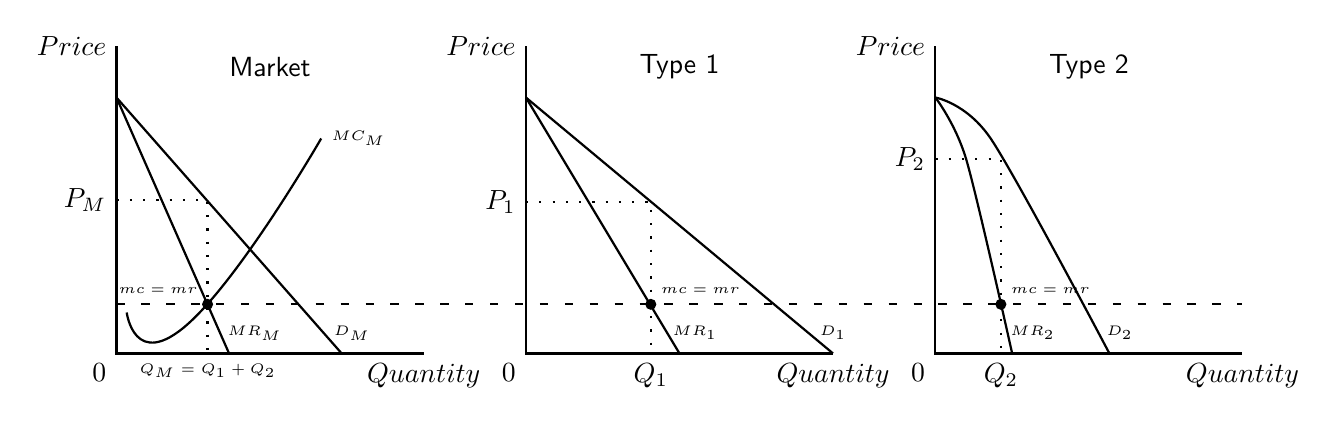
\begin{tikzpicture}[thick,font=\sffamily,scale=1.3]
	%axies
	\draw (-6,3) node[left]{$Price$} -- (-6,0) node[below left] {$0$} -- (-3,0) node[below]{$Quantity$}; %market
	\draw (-2,3) node[left]{$Price$} -- (-2,0) node[below left] {$0$} -- (1,0) node[below]{$Quantity$}; %type 1
	\draw (2,3) node[left]{$Price$} -- (2,0) node[below left] {$0$} -- (5,0) node[below]{$Quantity$}; %type 2
	
	%titles
	\node[] at (-4.5,2.8) {Market}; %Market title
	\node[] at (-0.5,2.8) {Type 1}; %Type 1 title
	\node[] at (3.5,2.8) {Type 2}; %Market title
	  
	 %market-----------------------------------------------
	\draw[] (-6,2.5) -- (-3.8,0); %demand
		\node[] at (-3.7,0.2) {\tiny{$D_{M}$}}; %Demand label
	\draw[] (-6,2.5) -- (-4.9,0); %mr
	\node[] at (-4.65,0.2) {\tiny{$MR_{M}$}}; %MR label
	\draw[] plot [smooth, tension=1] coordinates {(-5.9,0.4) (-5.3,0.29) (-4,2.1)}; %mc
	\node[right] at (-4,2.1) {\tiny{$MC_{M}$}}; %MC label
	\node[style={fill=black,circle,inner sep=0pt,minimum size=4pt}] at (-5.11,0.48) { }; %mc=mr node
	\node[above left]at (-5.11,0.48) {\tiny{$mc=mr$}}; %mc=mr label
	\draw[loosely dashed] (-6,0.48) -- (5,0.48); %mc line
	\draw[loosely dotted] (-6,1.5) node[left]{$P_{M}$} -| node[pos=0.25,below=3mm] {} (-5.11,0) node[below]{\tiny{$Q_{M}=Q_{1}+Q_{2}$}}; %dotted lines
	
	 %Type 1 - elastic-------------------------------------
	\draw[] (-2,2.5) -- (1,0); %demand
	\node[] at (1,0.2) {\tiny{$D_{1}$}}; %Demand1 label
	\draw[] (-2,2.5) -- (-0.5,0); %mr
	\node[] at (-0.35,0.2) {\tiny{$MR_{1}$}}; %MR1 label
	\node[style={fill=black,circle,inner sep=0pt,minimum size=4pt}] at (-0.78,0.48) { }; %mc=mr node
	\node[above right]at (-0.78,0.48) {\tiny{$mc=mr$}}; %mc=mr label	
	\draw[loosely dotted] (-2,1.48) node[left]{$P_{1}$} -| node[pos=0.25,below=3mm] {} (-0.78,0) node[below]{$Q_{1}$}; %dotted lines
	 
	 %Type 2 - inelastic------------------------------------
	%\draw[] (2,2.5) -- (3.5,0); %demand
	%\draw[] (2,2.5) -- (2.75,0); %mr
	\draw[] plot [smooth, tension=0.5] coordinates {(2,2.5) (2.54,2.1) (3.7,0)}; %demand
	\node[] at (3.8,0.2) {\tiny{$D_{2}$}}; %Demand2 label
	\draw[] plot [smooth, tension=0.5] coordinates {(2,2.5) (2.3,1.9) (2.75,0)}; %mr
	\node[] at (2.95,0.2) {\tiny{$MR_{2}$}}; %MR2 label
	\node[style={fill=black,circle,inner sep=0pt,minimum size=4pt}] at (2.64,0.48) { }; %mc=mr node
	\node[above right]at (2.64,0.48) {\tiny{$mc=mr$}}; %mc=mr label
	\draw[loosely dotted] (2,1.9) node[left]{$P_{2}$} -| node[pos=0.25,below=3mm] {} (2.64,0) node[below]{$Q_{2}$}; %dotted lines
\end{tikzpicture}
\end{document}